\documentclass[12pt,a4paper]{book}

% Formato del documento
%\usepackage[papersize={210mm,297mm},inner=3.5cm,outer=2cm,top=2.5cm,bottom=2.5cm]{geometry}
%\renewcommand{\baselinestretch}{1}
%\setlength{\parskip}{8pt}

\usepackage[utf8]{inputenc}
\usepackage{amssymb}
\usepackage{amsmath}
\usepackage{graphicx}
\usepackage{tikz}
\usepackage{tkz-graph}
\usepackage{hyperref}
\usepackage[parfill]{parskip}
\usepackage{float}
\renewcommand{\chaptername}{Capítulo}
\renewcommand{\contentsname}{Índice}
\renewcommand{\bibname}{Bibliografía}
\renewcommand{\figurename}{Figura}
\setcounter{chapter}{-1}

\definecolor{verde_oscuro}{rgb}{0.0, 0.5, 0.0}

\newtheorem{defi}{Definición}[section]
\newtheorem{prop}{Proposición}[section]
\newtheorem{propi}{Propiedades}[section]
\newtheorem{lema}{Lema}[section]
\newtheorem{tma}{Teorema}[section]
\newtheorem{cor}{Corolario}[section]
\newtheorem{nota}{Nota}[section]
\newtheorem{ejem}{Ejemplo}[section]

\hypersetup{
    colorlinks=true,
    linkcolor=blue,
    filecolor=magenta,      
    urlcolor=cyan,
    pdftitle={Overleaf Example},
    pdfpagemode=FullScreen,
    }

\urlstyle{same}

%%%%%%%ALTERNATIVA 2%%%%%%%%%%%%
\textheight=21cm
\textwidth=17cm
%\topmargin=-1cm
\oddsidemargin=0cm
\evensidemargin=0cm
\parindent=0mm
\pagestyle{plain}
%%%%%%%%%%%%%%%%%%%%%

%%%%%%%  Comando Portada  %%%%%%%%%%%
% Ajustes de geometría si la portada sigue sin caber
% \geometry{a4paper, top=1cm, bottom=1cm, left=1cm, right=1cm} 

\newcommand{\nuevaportada}[6]{
    \thispagestyle{empty}
    \begin{center}
        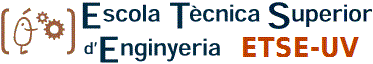
\includegraphics[width=0.5\textwidth]{images/logo.png}
        
        \vspace{0.3cm} % Espacio reducido
        {\Large\bfseries\textsc{M\'aster Universitario en #1}\par}
        
        \vspace{0.3cm} % Espacio reducido
        
\includegraphics[width=0.4\textwidth]{images/uv.png}
        
        \vspace{0.3cm} % Espacio reducido
        {\Large\bfseries\textsc{Trabajo de Fin de M\'aster}\par}
        
        \vspace{0.5cm} % Mantener este espacio un poco más grande para el título
        {\Large\bfseries #2\par}
        
        \vspace{1.5cm} % Reducido a 1.5cm desde 2cm
        \begin{flushright}
            \begin{tabular}{l} 
                {\large\bfseries\textsc{Autor:}} \\
                {\large\textsc{#3}} \\ [0.3cm] % Espacio reducido
                {\large\bfseries\textsc{Tutora:}} \\ 
                {\large\textsc{#4}} \\ [0.3cm] % Espacio reducido
                {\large\bfseries #5} 
            \end{tabular}
        \end{flushright}
    \end{center}
    % Eliminamos \clearpage de aquí, ya que la portada debe ser una sola página
    % Si necesitas un salto de página después de la portada, lo añades en el documento principal.
}

\begin{document}

\nuevaportada{Ciencia de Datos}{Resolución mediante GRASP y aprendizaje reforzado del Problema de Localización de k-Centros Balanceado Multiobjetivo}{Manuel Rubio Martínez}{Anna Martínez Gavara}{Abril, 2025}

\clearpage

\newpage
\tableofcontents

\newpage

\section*{Resumen}
Aquí va el contenido de tu resumen en español. Explica brevemente el objetivo, la metodología, los resultados y las conclusiones de tu TFM.

\newpage

\section*{Abstract}
Here goes the content of your abstract in English. Briefly explain the objective, methodology, results, and conclusions of your TFM.

\newpage

\section*{Resum}
Aquí va el contingut del teu resum en valencià. Explica breument l'objectiu, la metodologia, els resultats i les conclusions del teu TFM.

\newpage

\chapter{Introducción}

\section{Introducción al TFM}
En este Trabajo de Fin de Máster se va a estudiar, mediante un algoritmo GRASP con técnicas de Aprendizaje Reforzado, la resolución del problema de localización de k-centros balanceado multiobjetivo.
Se ha tomado como referencia \cite{k-balanced_1}, enunciando y resolviendo el problema, junto a la publicación posterior \cite{k-Balanced_2}, donde se desarrollaron nuevos métodos de resolución utilizando GRASP y Path Relinking.

Se han tomado las mismas consideraciones a la hora de definir el problema, y se han trabajado los mismos datos sintéticos.
Más adelante se compararán dos implementaciones distintas del algoritmo, contrastando sus resultados con los obtenidos en los artículos previos.

El objetivo principal será evaluar si la implementación de modelos de aprendizaje no supervisado en algoritmos metaheurísticos puede mejorar significativamente su rendimiento.

Esta introducción se centrará en contextualizar el área de la optimización, revisando brevemente su evolución histórica, las definiciones clave y los principales enfoques utilizados para descomponer y abordar problemas de esta naturaleza. También se añadirán los conceptos básicos para entender cómo funciona el Aprendizaje Reforzado.


\section{Historia de la optimización}
El origen de la optimizacaión se remonta a la antigua Grecia, donde matemáticos como Euclides o Arquímedes la utilizaban en busca de soluciones a problemas del área de la geometría.

La versión que conocemos hoy en día no empezó a desarrollarse hasta el siglo XVII, con la aparición del cálculo diferencial, impulsado por los trabajos de Isaac Newton y Gottfried Wilhelm Leibniz\cite{Leibniz}. Con él se empezaron a estudiar las funciones y sus puntos extremos,
en los cuales, bajo ciertas condiciones, pueden encontrarse los valores óptimos.

No encontramos grandes avances hasta mediados del siglo XX cuando, fruto de la necesidad de resolver problemas logísticos durante la Segunda Guerra Mundial, el matemático George Bernard Dantzig \cite{Dantzig} desarrolló la programación lineal, la cual sentó las bases para el posterior surgimiento tanto de la programación no lineal, como de la entera y la dinámica.

A pesar de todo, la mayoría de problemas del mundo real, especialmente aquellos que dependen de un gran número de variables, con funciones objetivo complejas y restricciones no lineales, acaban siendo demasiado costosos computacionalmente. Esta inviabilidad de los métodos de obtención de soluciones exactas propició el surgimiento de los metaheurísticos.

Los algoritmos metaheurísticos\cite{metaheuristicos}, acuñados por el especialista en ciencias de la computación Fred Glover,
son la alternativa realista para la búsqueda de soluciones aproximadas, pero cercanas al óptimo, en un tiempo aceptable.

Las metaheurísticas son fundamentales en Ciencia de Datos, ya que permiten abordar de manera eficiente problemas complejos presentes en:

\begin{itemize}
    \item \textbf{Clustering:} El algoritmo \textbf{k-means} particiona el espacio de observaciones en un número determinado de clústeres (grupos) y determina qué observaciones pertenecen a cada uno de ellos. 
    Si intentásemos encontrar la solución exacta, sería computacionalmente muy costoso, y la naturaleza del algoritmo hace que la solución sea dependiente de los grupos iniciales (generados aleatoriamente), pudiendo caer en óptimos locales.
    Las metaheurísticas ayudan a solventar estos problemas al proporcionar estrategias más robustas de exploración del espacio de soluciones.
    
    \item \textbf{Selección de variables:} En la construcción de modelos de predicción, solemos encontrarnos con un número elevado de variables, por lo que definir el modelo con base en todas ellas no es factible. Mediante metaheurísticos podemos 
    reducir significativamente la dimensión del espacio, utilizando un subespacio con las variables que mejor sirvan al modelo.
    
    \item \textbf{Ajuste de hiperparámetros:} Modelos de inteligencia artificial como las redes neuronales necesitan ajustar sus hiperparámetros para ser eficaces (número de capas, tasa de aprendizaje, etc.). Este ajuste constituye también un problema de optimización en espacios de búsqueda de alta dimensión, frente a métodos tradicionales como la \textit{búsqueda en cuadrícula} (\textit{grid search}), los metaheurísticos ofrecen una alternativa más eficiente y flexible.
\end{itemize}



En esencia, la optimización es el proceso de encontrar las mejores soluciones para un problema determinado, de la forma más eficiente y precisa posible.
Cualquier reto que se enmarque en esta búsqueda de un resultado óptimo puede considerarse, por tanto, un problema de optimización.

Si bien esta idea es intuitiva, el rigor matemático exige una definición más precisa.

\section{Formulación Matemática}

Para expresar un problema de optimización de forma matemática, definimos las tres partes en las que se puede descomponer:

\begin{itemize}
    \item \textbf{Variables de Decisión:} Son las incógnitas del problema, los valores que deberemos modificar para obtener la solución o soluciones óptimas. Se representan como un vector $\mathbf{x} = (x_1, x_2, \ldots, x_n)$, donde $n$ es el número de variables.

    \item \textbf{Función Objetivo:} Función que se desea minimizar o maximizar.\\
    Se denota comúnmente como $f(\mathbf{x})$, donde $f$ es la función que establece la relación entre las variables ($\mathbf{x}$) y el objetivo que deseamos optimizar.
    Por ejemplo:
    $$ \min_{\mathbf{x}} f(\mathbf{x}) \quad \text{o} \quad \max_{\mathbf{x}} f(\mathbf{x}) $$
    La función $f: \mathbb{R}^n \to \mathbb{R}$ mapea el vector de variables a un valor escalar, el cual buscaremos mejorar.

    \item \textbf{Restricciones:} Son las condiciones o limitaciones que deben satisfacer las variables de decisión. Pueden ser de igualdad o de desigualdad. Se expresan generalmente como:
    \begin{align*}
        g_i(\mathbf{x}) &\le 0 & \quad \text{para } i = 1, \ldots, m \\
        h_j(\mathbf{x}) &= 0 & \quad \text{para } j = 1, \ldots, p
    \end{align*}
    Donde $g_i(\mathbf{x})$ son las $m$ restricciones de desigualdad y $h_j(\mathbf{x})$ son las $p$ restricciones de igualdad.
    En caso de tener restricciones del tipo $g_k(\mathbf{x})\geq0$, se puede transformar a $\leq$ sabiendo que $-g_k(\mathbf{x}) \leq 0$.
    
    Además de restricciones funcionales, también pueden existir restricciones sobre el dominio de las variables, como $x_k \ge 0$ (variables no negativas),  $x_k \in \{0,1\}$ (variables binarias) o $x_k \in \mathbb{Z}$ (variables enteras).
\end{itemize}

Ahora sí, pasadas las definiciones previas, un problema completo de optimización se formula de la siguiente manera:
$$
\begin{array}{ll}
\text{Minimizar (o Maximizar)} & f(\mathbf{x}) \\ \\
\text{Sujeto a:} & g_i(\mathbf{x}) \le 0, \quad i = 1, \ldots, m \\
& h_j(\mathbf{x}) = 0, \quad j = 1, \ldots, p \\
& \mathbf{x} \in X
\end{array}
$$
Donde $X$ representa el conjunto de factibilidad o dominio de las variables de decisión.

Ahora vamos a clasificar los problemas de optimización según 2 características principales.

\subsection{Optimización Lineal vs. No Lineal}

La primera distinción la haremos según la naturaleza de las funciones involucradas, tanto en la función objetivo como en las restricciones. En general, esto determinará si el problema puede ser resuelto fácilmente de manera exacta o si requerirá de métodos más complejos con soluciones aproximadas.

\subsubsection{Optimización Lineal}
Diremos que un problema es de \textbf{optimización lineal} cuando, tanto la función objetivo como todas las funciones de las restricciones, son lineales con respecto a las variables de decisión. 

Características principales:
\begin{itemize}
    \item La función objetivo tiene la forma $f(\mathbf{x})=c_1x_1+c_2x_2+...+c_nx_n$ donde los $c_i \in \mathbb{R} \quad \forall i \in 1,2,...,n$.
    \item Todas las restricciones son lineales, con la forma $a_1x_1+a_2x_2+...+a_nx_n\leq b$ o $=b$, donde $a_i \in \mathbb{R} \quad \forall i \in 1,2,...,n$ y $b\in \mathbb{R}$.
    \item Estas condiciones hacen que el conjunto de soluciones factibles ($X$) tenga la forma de un poliedro convexo, lo que simplifica la búsqueda de la solución óptima.
    \item El algoritmo Simplex, propuesto en \cite{Dantzig1951}, es el más extendido para resolver este tipo de problemas y garantiza encontrar el óptimo global, si existe.
\end{itemize}

\subsubsection{Optimización No Lineal}
Diremos que un problema es de \textbf{optimización no lineal} cuando al menos una de sus funciones (objetivo o de restricción) es no lineal (con respecto a sus variables de decisión). 

Características principales:
\begin{itemize}
    \item La función objetivo $f(\mathbf{x})$ o alguna de sus restricciones $g_i(\mathbf{x})$ o $h_j(\mathbf{x})$ contiene términos no lineales. Por ejemplo:
    $$f(\mathbf{x})=2x_1^2+5x_2^7-\ln(x).$$
    \item El conjunto de soluciones factibles puede ser no convexo, lo que deriva en múltiples óptimos locales y el aumento de la complejidad del problema a la hora de buscar el óptimo global.
    \item La mayoría de algoritmos para resolverlos suelen utilizar técnicas de búsqueda local y no garantizan encontrar el óptimo global.
\end{itemize}

Ejemplos:
\begin{itemize}
    \item \textbf{Lineal:} Una fábrica busca maximizar su beneficio produciendo varios artículos, donde cada uno consume una cantidad fija de recursos (horas de máquina, materia prima) y genera un beneficio fijo, con restricciones de recursos y uso de las máquinas.
    \item \textbf{No lineal:} Encontrar los parámetros de una curva que se ajustan a unos datos concretos, minimizando el error cuadrático medio entre la aproximación (la curva) y el valor exacto de los datos.
\end{itemize}


\subsection{Optimización Discreta vs. Continua}
la segunda característica a estudiar será la naturaleza de sus variables de decisión. Que sean continuas o discretas
limitará en gran medida el tipo de algoritmos que puedan utilizarse para resolverlos.

\subsubsection{Optimización Continua}
En la optimización continua, las variables de decisión pueden tomar cualquier valor real dentro de su dominio o rango permitido. Es decir, no están restringidas a tomar valores enteros, a un conjunto finito o a un conjunto numerable de posibles soluciones. Esto las hace adecuadas para modelar fenómenos que varían de forma suave, como el tiempo, el espacio, la temperatura, etcétera.

Características principales:
\begin{itemize}
    \item Variables pertenecientes a un espacio continuo, típicamente $\mathbb{R}^n$.
    \item Las funciones objetivo $f(\mathbf{x})$ y sus restricciones $g_i(\mathbf{x}), \;h_j(\mathbf{x})$ suelen ser continuas y diferenciables.
    \item Las técnicas de resolución a menudo involucran cálculo diferencial para encontrar el mejor camino de mejora de la solución.
\end{itemize}

\subsubsection{Optimización Discreta}
En este caso, las variables de decisión están restringidas a tomar valores de un conjunto finito o, al menos, numerable. Los casos más comunes son variables restringidas a tomar valores enteros $(0,1,2,...)$, binarios $(0,1)$ o variables que representan la elección de elementos de un conjunto específico (por ejemplo, el ``trabajador 1'' o el ``trabajador 2'').

Características principales:
\begin{itemize}
    \item Las variables pertenecen al espacio discreto.
    \item No se pueden utilizar directamente las técnicas de cálculo diferencial que, en cambio, sí se podrían usar en el espacio continuo.
    \item Los problemas suelen ser más complejos de resolver y computacionalmente más costosos, por lo que suelen requerir algoritmos específicos como la programación entera, la programación dinámica o métodos combinatorios para poder resolverlos.
\end{itemize}

Ejemplos:
\begin{itemize}
    \item Como casos continuos, tenemos el diseño de la aerodinámica de un avión (modelado de los parámetros de las curvas de la superficie) o la velocidad óptima de un vehículo para reducir su consumo de combustible.
    \item Como casos discretos, tenemos el problema de la mochila (escoger el mayor valor en elementos de un conjunto sin exceder una capacidad dada) o la planificación de rutas.
\end{itemize}

Para esta primera parte de caracterización de la optimización he tomado como referencia el libro \cite{Numerical_optimization_nocedal_wright} de Numerical Optimization de Jorge Nocedal y Stephen J. Wright.

Para concluir la parte teórica de la optimización, voy a concretar tanto la rama a la que pertenece el problema de k-centros balanceado (la optimización \textbf{combinatoria}) como lo que significa que sea \textbf{multiobjetivo}

\subsection{Optimización Combinatoria}
La optimización combinatoria se centra en encontrar la solución óptima dentro de un conjunto de soluciones finito o numerable. Aunque la cantidad de soluciones posibles pueda ser finita, no significa que el problema sea sencillo.
De hecho, la mayoría de estos problemas de optimización entran dentro de los denominados problemas \textbf{NP-difíciles}\cite{np_hard}.

Que sean NP-difíciles implica que el tiempo necesario para encontrar la solución óptima crece exponencialmente a medida que aumenta el tamaño del problema. Esto hace que la búsqueda exhaustiva de la solución sea computacionalmente inviable para la mayoría de los casos de estudio en el mundo real.

\textbf{Características principales:}
\begin{itemize}
    \item \textbf{Espacio de soluciones discreto:} Las variables de decisión están restringidas a un conjunto finito o numerable de valores, como la selección o no de un elemento, o la ordenación de un conjunto. Se puede decir que entran dentro de los casos de \textbf{optimización discreta}. 
    \item \textbf{Complejidad computacional elevada:} A menudo, el número de soluciones posibles es astronómicamente grande, lo que requiere algoritmos especializados para explorar el espacio de búsqueda de manera eficiente.
    \item \textbf{Estructura del problema:} Las técnicas de resolución aprovechan la estructura combinatoria subyacente del problema, utilizando métodos como la programación entera, la teoría de grafos o los algoritmos metaheurísticos.
\end{itemize}

Sentada la base teórica, ahora podemos definir correctamente el problema.

El problema de localización de k-centros balanceado consiste en seleccionar, de un conjunto de $m$ posibles centros, los $k$ que mejoren su función o funciones objetivo. El número total de posibles soluciones es finito, y viene dado por el coeficiente binomial 
$$ \binom{m}{k} = \frac{m!}{(m-k)!k!}$$

Para ilustrar la explosión combinatoria, consideremos el caso con $m=50$ y $k=5$. El número de combinaciones posibles sería:

$$
    \binom{50}{5} = \frac{50!}{(50-5)!5!} = 2,118,760.
$$

Pasando a problemas más realistas, si tenemos $m=1000$ posibles emplazamientos, y $k=50$ centros a construir, la cantidad de soluciones posibles se dispara a una cifra del orden de $2.28 \times 10^{120}$. 
Evaluar cada una de estas soluciones para encontrar la óptima de forma exacta es una tarea imposible, incluso para los superordenadores más potentes, ya que requeriría tiempos de computación demasiado elevados.

Otros ejemplos clásicos de optimización combinatoria incluyen el \textbf{Problema del Viajante de Comercio (TSP)}, 
que busca la ruta más corta que visita un conjunto de ciudades una sola vez;
el \textbf{problema de la mochila}, que consiste en seleccionar los objetos más valiosos sin superar una capacidad de peso;
o la \textbf{planificación de horarios}, donde se asignan recursos (como aulas o profesores) a franjas horarias para satisfacer un conjunto de restricciones.

\subsection{Optimización Multiobjetivo}

Definir la cantidad de funciones objetivo que se van a utilizar para modelizar el problema consituye una de las características más relevantes y, a menudo, más complejas del mismo, debido a su naturaleza inherentemente subjetiva.
¿Debe considerarse únicamente una función objetivo? ¿O hay que tener en cuenta simultáneamente 
dos o más funciones objetivo? Si bien enfocarse en una única función facilita el análisis y su resolución, rara vez refleja la complejidad de los problemas reales. La optimización multiobjetivo
abordará los problemas mejorando simultáneamente dos o más funciones objetivo que, a menudo, estarán en conflicto entre sí. Mejorar una solerá implicar el empeoramiento de la otra.
Por ejemplo, en el diseño de un vehículo, minimizar el consumo de combustible (objetivo 1) estará en conflicto con maximizar la potencia del motor (objetivo 2).

La optimización multiobjetivo permite abordar este tipo de situaciones analizando\\
explícitamente las compensaciones o \textit{trade-offs} entre los diferentes objetivos. En lugar de proporcionar una única solución, esta técnica ofrece un conjunto de soluciones eficientes y equilibradas que permiten
tomar decisiones evaluando distintas alternativas y elegir la que mejor se adapte a las necesidades del problema.

En este contexto, el concepto de “solución óptima” deja de ser aplicable. En su lugar, se busca identificar un conjunto de soluciones que representen las mejores compensaciones posibles entre los objetivos. Este conjunto se denomina \textbf{Frente de Pareto}.

Una solución se considera \textbf{no dominada} (u óptima en el sentido de Pareto) si no existe otra solución factible que la supere en al menos un objetivo sin empeorar en ninguno de los demás. El Frente de Pareto está compuesto por todas las soluciones no dominadas del espacio de soluciones factibles.
\begin{figure}[H]
    \centering
    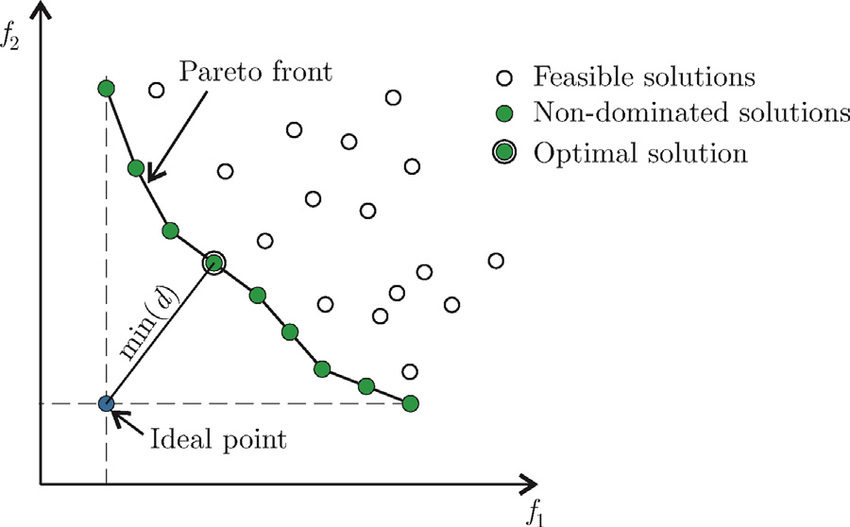
\includegraphics[width=0.6\textwidth]{images/pareto_front.png}
    \caption{\cite{Bre2017} Ilustración de un frente de pareto para un problema de minimización con dos objetivos ($f_1, f_2$). Las soluciones en verde son óptimas y pertenecen al Frente de Pareto, ya que no se puede mejorar un objetivo sin empeorar el otro. El punto ideal, que estaría en la parte inferior izquierda de la gráfica, sería la mejor solución imaginable combinando lo mejor de todas las soluciones. Las soluciones sin colorear están dominadas por alguna de las verdes.}
    \label{fig:pareto}
\end{figure}

Una vez definidos los problemas de optimización, ahora viene la parte más importante, cómo resolverlos.

\section{Resolución de Problemas de Optimización Multiobjetivo}

\subsection{Métodos Exactos}

Los métodos exactos para la optimización multiobjetivo tienen como finalidad encontrar el Frente de Pareto al completo. Sin embargo, al igual que en sus contrapartes mono-objetivo, se enfrentan al mismo obstáculo: la complejidad computacional. La mayoría de estos problemas son \textbf{NP-difíciles}.

No obstante, para problemas sencillos, con pocas variables y reducido espacio de soluciones, se pueden resolver con los siguientes métodos:

\begin{itemize}
    \item \textbf{Métodos de Ponderación (Weighted Sum):} Transforman el problema multiobjetivo en problemas mono-objetivo, asignando pesos a cada una de las funciones objetivo y sumándolos para crear una única función agregada. Al variar sistemáticamente los pesos, se pueden ir generando las soluciones del Frente de Pareto. Sin embargo, este método no garantiza encontrar todas las soluciones si el frente tiene una forma no convexa.

    \item \textbf{Método de las Restricciones Épsilon ($\epsilon$-constraint):} Consiste en optimizar una de las funciones objetivo, convirtiendo el resto en restricciones que limitan su valor a un máximo $\epsilon$.\\
    Modificando los valores de $\epsilon$ para cada objetivo-restricción, se puede explorar y reconstruir el Frente de Pareto. A diferencia del método de ponderación, este sí puede encontrar soluciones en frentes no convexos.

    \item \textbf{Algoritmos de Ramificación y Acotación (Branch and Bound) Multiobjetivo:} Estos algoritmos extienden el clásico \textit{Branch and Bound}. El proceso de ramificación es similar (se divide el problema en subproblemas más pequeños), pero la fase de acotación (o poda) es más compleja. En lugar de usar una única cota, se trabaja con conjuntos de cotas (un vector por cada objetivo). Una rama del árbol de búsqueda se poda solo si se puede demostrar que no puede contener ninguna solución no dominada en comparación con las soluciones ya encontradas.

    \item \textbf{Algoritmos de Ramificación y Corte (Branch and Cut) Multiobjetivo:} De manera análoga, esta técnica extiende \textit{Branch and Cut}. Se añaden planos de corte (restricciones adicionales) no solo para mejorar la relajación del problema mono-objetivo, sino para refinar la aproximación del espacio de soluciones factibles en el dominio multiobjetivo, permitiendo podar ramas del árbol de búsqueda de forma más eficiente.
\end{itemize}

\subsection{Metaheurísticas}
Como se indicó al principio del capítulo, las metaheurísticas\cite{metaheuristicos} aparecen con el desarrollo de las ciencias de la computación como principal solución a los problemas de optimización complejos. Allí donde los métodos exactos no serían capaces de encontrar el óptimo,
los algoritmos metaheurísticos buscan soluciones "buenas" en tiempos de ejecución razonables, sacrificando la garantía de optimalidad global que proporcionan los métodos exactos.

Generalmente combinan heurísticas con aleatoriedad para obtener soluciones de calidad, a la vez que se explora el espacio buscando nuevos óptimos locales.\\
Estos métodos combinan dos estrategias:
\begin{itemize}
    \item \textbf{Exploración:} Capacidad de recorrer diversas áreas del espacio de búsqueda para encontrar nuevas soluciones, evitando quedar atrapado en óptimos locales.
    \item \textbf{Explotación:} Capacidad de intensificar la búsqueda en una región prometedora para encontrar los mejores óptimos locales dentro de ella.
\end{itemize}

Son algoritmos muy generales, fáciles de implementar y adaptables a casi 
cualquier problema de optimización. Los principales algoritmos metaheurísticos son:
\begin{itemize}
    \item \textbf{Algoritmos Genéticos (GA - Genetic Algorithms)}\\
    Inspirados en la selección natural y la genética, se basan en la generación aleatoria de soluciones y en el cruce de las más prometedoras entre sí, 
    mientras se añaden mutaciones (pequeñas modificaciones en las soluciones) para aportar diversidad.
    
    \item \textbf{Recocido Simulado (SA - Simulated Annealing)}\\
    Basado en un proceso físico, simula el recocido de metales (calentarlos y enfriarlos para alterar su estructura). Explora soluciones aceptando movimientos de mejora, pero también aquellos que puedan empeorar la solución, 
    en función de una probabilidad dependiente de una variable ``temperatura", que decrece con el paso de las iteraciones. En fases tempranas, una temperatura alta favorece la exploración, mientras que en fases finales una temperatura baja favorece la explotación.
    
    \item \textbf{Búsqueda Tabú (TS - Tabu Search)}\\
    Genera una lista ``tabú'' que actúa como memoria a corto plazo del algoritmo, incluyendo los movimientos recientes con el objetivo de no repetir soluciones y así forzar la exploración de nuevas zonas, aunque eso conlleve aceptar movimientos que no sean los mejores posibles.
    
    \item \textbf{Optimización por Colonia de Hormigas (ACO - Ant Colony Optimization)}\\
    Diseñado originalmente para problemas de rutas, construye soluciones iterativamente a través de un grafo, cuyas aristas se van ponderando a medida que se generan soluciones de calidad.
    
    \item \textbf{GRASP (Greedy Randomized Adaptive Search Procedure)}\\
    Algoritmo fundamentado en dos fases. Una primera de construcción, en la que se genera una solución mediante un proceso aleatorizado, y una segunda de búsqueda local, en la que se intenta mejorar la solución generada.
\end{itemize}

\section{Aprendizaje Reforzado}

El Aprendizaje Reforzado \cite{intro_reforzado} (del inglés, \textit{Reinforcement Learning} o RL) es un área del aprendizaje automático inspirada en la psicología conductista. Se utiliza en problemas donde un agente debe tomar acciones en un entorno dinámico con el objetivo de maximizar una cierta recompensa.\\
A diferencia de otros paradigmas de la ciencia de datos como el aprendizaje supervisado, donde los algoritmos aprenden de un conjunto de datos etiquetado, en RL el agente aprende por sí mismo a través de la experiencia directa, en un proceso de prueba y error. 

El objetivo del RL no es encontrar la respuesta correcta, sino descubrir una estrategia de actuación óptima que maximice la recompensa a largo plazo. Por esta razón, el RL se considera un problema de optimización secuencial de decisiones.

El agente busca optimizar su comportamiento para lograr un objetivo a largo plazo, lo que lo convierte en una herramienta excepcionalmente potente para resolver problemas complejos en dominios como la robótica, la gestión de la cadena de suministro, las finanzas algorítmicas o incluso para resolver los propios problemas de optimización combinatoria.

\subsection{Componentes Clave del Aprendizaje Reforzado}

Todo problema de Aprendizaje Reforzado se modela a través de los siguientes elementos:

\begin{itemize}
    \item \textbf{Agente}: Entidad que aprende del entorno y toma las decisiones. Puede ser un robot que aprende a caminar, un programa que juega al ajedrez o un sistema de gestión de tráfico urbano.
    \item \textbf{Entorno}: Es el mundo, real o simulado, donde se encuentra e interactúa el agente. Este únicamente puede tener control parcial del entorno.
    \item \textbf{Tiempo ($T$)}: Momentos discretos en los que se desarrolla el Aprendizaje Reforzado ($t=0, 1, 2, \dots$).
    \item \textbf{Estado ($S$)}: Descripción de la situación del entorno. Representa toda la información relevante que el agente puede necesitar para la toma de decisiones. $S_t$ representa el entorno en el momento $t$.
    \item \textbf{Acción ($A$)}: Es el conjunto de las posibles decisiones que el agente puede tomar. $A_t$ representa la acción tomada en el momento $t$.
    \item \textbf{Recompensa ($R$)}: Señal numérica que el entorno devuelve al agente tras cada acción. La recompensa indica cómo de buena o mala ha sido la acción tomada al transitar al nuevo estado $S_{t+1}$. El objetivo del agente es maximizar la suma de estas recompensas a lo largo del tiempo. $R_t$ es la recompensa obtenida en el momento $t$.
\end{itemize}

El proceso de aprendizaje se desarrollaría de la siguiente manera:
\begin{enumerate}
    \item El agente observa el estado actual del entorno, $S_t$.
    \item Basándose en $S_t$, el agente elige una acción, $A_t$.
    \item El entorno recibe la acción $A_t$ y, como resultado, transita a un nuevo estado, $S_{t+1}$.
    \item El entorno emite una recompensa, $R_{t+1}$, al agente.
\end{enumerate}
Este ciclo iterativo genera una trayectoria de estados, acciones y recompensas que el agente utilizará para aprender una política que maximice su rendimiento a largo plazo.

El objetivo del agente no es maximizar la recompensa inmediata, sino el \textbf{retorno} (o recompensa acumulada), denotado como $G_t$.
El retorno es la suma de todas las recompensas futuras a partir del instante $t$. 
Para evitar sumas infinitas en tareas continuas y para dar más importancia a las recompensas cercanas en el tiempo, se introduce un factor de descuento $\gamma$, donde $0 \le \gamma \le 1$.

El \textbf{retorno descontado} se define como:
\[ G_t = R_{t+1} + \gamma R_{t+2} + \gamma^2 R_{t+3} + \dots = \sum_{k=0}^{\infty} \gamma^k R_{t+k+1} \]

\begin{itemize}
    \item Si $\gamma = 0$, el agente solo tiene en cuenta la recompensa inmediata.
    \item Si $\gamma$ se acerca a 1, el agente valora las recompensas futuras casi tanto como las inmediatas.
\end{itemize}

El problema de optimización en RL consiste en encontrar una estrategia que maximice el valor esperado de este retorno. Para encontrarla, volvemos a tener el dilema que encontramos a la 
hora de definir las metaheurísticas.

\subsection{Exploración vs. Explotación}

Para que un agente aprenda la manera  óptima qué acciones tomar, deberá equilibrar la explotación y la exploración:
\begin{itemize}
    \item \textbf{Explotación}: Utilizar el conocimiento actual para tomar la mejor acción conocida y maximizar la recompensa inmediata.
    \item \textbf{Exploración}: Probar nuevas acciones, potencialmente subóptimas, para descubrir si pueden conducir a recompensas mayores a largo plazo y mejorar su conocimiento del entorno.
\end{itemize}
Si únicamente explota, se arriesga a quedar atascado en un óptimo local.\\
Si solo explora, obtendrá un rendimiento bajo al no aprovechar las buenas acciones que ha descubierto previamente.

El dilema se suele solventar siguiendo una estrategia \textbf{$\epsilon$-greedy (épsilon-voraz)}, donde el agente elige la mejor acción conocida con probabilidad $1-\epsilon$ (explotación) y una acción aleatoria con probabilidad $\epsilon$ (exploración).

\subsection{Ejemplos de Aplicación del Aprendizaje por Refuerzo}

\subsubsection{El Problema del Multi-Armed Bandit (Bandido de múltiples brazos)}

El problema del Multi-Armed Bandit (MAB) \cite{MAB} es un ejemplo clásico que ilustra perfectamente el dilema de exploración vs. explotación. Imaginemos a un jugador en un casino frente a $k$ máquinas tragaperras (los ``bandidos").
Cada máquina $i$ tiene una probabilidad desconocida $p_i$ de dar una recompensa. El objetivo del jugador es maximizar su ganancia total en un número limitado de jugadas.

\begin{itemize}
    \item \textbf{Agente}: El jugador.
    \item \textbf{Acciones}: Elegir una de las $k$ máquinas para jugar.
    \item \textbf{Recompensa}: 1 si la máquina da premio, 0 si no.
    \item \textbf{Estado}: En su formulación más simple, este problema no tiene diferentes estados, ya que la decisión sobre qué máquina jugar no depende de una configuración previa del entorno.
\end{itemize}

¿Debería el jugador seguir jugando con la máquina que, hasta ahora, ha dado los mejores resultados (explotación), o debería probar otras máquinas que podrían tener una tasa de pago aún mayor (exploración)?

Una solución siguiendo la política $\epsilon$-greedy sería:
\begin{enumerate}
    \item Estimar el valor esperado para cada una de las máquinas en $A$ (la recompensa media obtenida por cada una de ellas).
    \item Con probabilidad $1-\epsilon$, elegir la máquina $A_i \in A$ que haya generado una mayor recompensa media.
    \item Con probabilidad $\epsilon$, elegir una máquina al azar.
\end{enumerate}

Este sistema se suele utilizar en ensayos clínicos para asignar pacientes a diferentes tratamientos.

\subsubsection{Juegos de Estrategia}

Se utiliza incluso en juegos de estrategia complejos como el ajedrez, Go o videojuegos.

\begin{itemize}
    \item \textbf{Agente}: El programa que juega.
    \item \textbf{Estado}: La configuración actual del tablero o la pantalla del juego.
    \item \textbf{Acciones}: Los movimientos legales de las piezas o los comandos del mando.
    \item \textbf{Recompensa}: +1 por ganar la partida, -1 por perder y 0 por cada movimiento que no termine la partida.
\end{itemize}

Sistemas como AlphaGo \cite{AlphaGo} de DeepMind utilizaron RL para aprender a jugar a Go a un nivel sobrehumano.
El agente juega millones de partidas contra sí mismo, explorando el espacio de estrategias y entrenando una función de valor que le permita evaluar la calidad de cualquier posición del tablero.


\section{Resumen de los capítulos}
El presente Trabajo de Fin de Máster se estructura en cuatro capítulos, además de un apartado de agradecimientos y un anexo con definiciones necesarias para entender el trabajo.
En el capítulo 1 se presenta el Problema de Localización de k-Centros Balanceado, introduciendo el marco general de los problemas de localización, la motivación de este estudio y el modelo matemático para resolverlo.
El capítulo 2 expone la justificación de la elección de la metaheurística GRASP para abordar el problema, describe su implementación y detalla la incorporación del Aprendizaje Reforzado, mediante Multi-Armed Bandits (MAB).
El capítulo 3 recoge el diseño experimental y el análisis de los resultados obtenidos, comparando el rendimiento del algoritmo GRASP con y sin refuerzo frente a soluciones reportadas en estudios previos.
Finalmente, el capítulo 4 presenta las conclusiones derivadas del trabajo, así como posibles líneas de investigación futura.

\chapter{Problema de Localización de k-Centros Balanceado Multiobjetivo}

Ya podemos entrar en definir el problema que queremos abordar. Explicaré brevemente en lo que consisten los problemas de localización, sectores claves que requieres de soluciones a 
estos problemas, los principales modelos que se han realizado para resolverlos y la motivación junto al modelo propuesto para resolver el problema de localización de k-centros balanceado multiobjetivo.

\section{Problemas de Localización (Facility Location Problems)}

Los \textbf{problemas de localización de instalaciones} (\textit{Facility Location Problems}) constituyen una de las clases más relevantes dentro de la optimización combinatoria. Su objetivo es determinar las \textbf{ubicaciones óptimas} donde instalar infraestructuras como almacenes, hospitales, escuelas o antenas de telecomunicaciones.

Estos problemas suelen centrarse en algunos  delos siguientes objetivos:
\begin{itemize}
    \item \textbf{Minimizar los costes} o las distancias (ya sea la distancia total o la máxima entre instalaciones y clientes).
    \item \textbf{Maximizar beneficios} o el área de cobertura alcanzada.
    \item \textbf{Mejorar la equidad} del servicio o los tiempos de respuesta.
    \item \textbf{Equilibrar el uso} entre las distintas instalaciones.
\end{itemize}

Para encontrar la solución óptima, en estos problemas también se deben considerar \textbf{restricciones} prácticas, como la capacidad de cada centro, los límites presupuestarios o la necesidad de cubrir un mínimo de demanda.

La resolución de estos problemas es vital en \textbf{logística y cadena de suministro}, donde ubicar estratégicamente almacenes y centros
de distribución reduce drásticamente los costes de transporte y mejora la eficiencia de entregas, en el \textbf{sector sanitario}, para el cual ubicar hospitales y centros de atención primaria es crítico para
asegurar la máxima cobertura y accesibilidad de los mismos a toda la población, u en otros servicios públicos como la \textbf{planificación de escuelas}, \textbf{estaciones de bomberos} o \textbf{ubicación de bocas de metro}.

Algunas de las soluciones propuestas en la literatura se basan en los siguientes modelos:

\subsubsection{P-Mediana (p-median)}
El objetivo de este modelo es seleccionar $p$ ubicaciones de manera que se \textbf{minimice la suma total de las distancias} entre cada cliente y la instalación que se le asigna. Su enfoque está orientado a optimizar la \textbf{eficiencia global del sistema}, lo que lo convierte en una herramienta idónea para reducir los costes totales de transporte.
Se utiliza para determinar la ubicación de $p$ almacenes minimizando los costes de distribución, o para ubicar los $p$ centros de reciclaje reduciendod la distancia total recorrida por los vehículos de recogida.

\subsubsection{K-Centro (k-center)}
En este modelo, el objetivo es seleccionar $k$ ubicaciones para \textbf{minimizar la máxima distancia} que cualquier cliente debe recorrer hasta la instalación más cercana. Se trata de un enfoque centrado en la \textbf{equidad}, ya que busca optimizar el ``peor caso''. Es especialmente relevante en el diseño de servicios de respuesta rápida o de carácter crítico.
Su uso es clave en localizar qué $k$ hospitales se construyen para que el máximo tiempo de llegada ante una emergencia sea lo menor posible, o al ubicar las $k$ estaciones de bomberos, con el objetivo de que puedan responder
en situaciones remotas lo más rápido posible.

\subsubsection{Problemas de Cobertura (Coverage)}
Estos modelos tienen como propósito \textbf{maximizar la demanda atendida} dentro de un radio de servicio predefinido.

\paragraph{Location Set Covering Problem (LSCP)}
Su objetivo es \textbf{minimizar el número de instalaciones} necesarias para cubrir todos los puntos de demanda.
Se utiliza para determinar el número mínimo de escuelas de forma que todos los estudiantes vivan a menos de 2 km de una de ellas.


\paragraph{Maximal Covering Location Problem (MCLP)}
En este caso, el objetivo es \textbf{maximizar la demanda cubierta} con un número fijo $p$ de instalaciones, lo que resulta especialmente útil cuando no es posible cubrir a toda la población.
Es necesario para casos en los que se selecciona la ubicación de $p$ bibliotecas móviles para dar servicio al mayor número posible de ciudadanos.



\section{Motivación}

\section{Modelo Matemático}



\chapter{Resolución del problema}
Aquí metería una breve introducción a lo que voy a utilizar.

\section{Por qué el GRASP}
- Es un método sencillo de implementar, pero complicado de adaptar para realizar un buen desempeño
- Suele obtener buenas soluciones muy rápido, al contrario que Tabu o Algoritmos Genéticos
- Es especialmente bueno para problemas combinatorios, ya que las búsquedas locales son más fáciles de definir

\section{Metaheurísticas del grasp}
definir primero la monoobjetivo, cómo se comporta, y por qué en monoobjetivo es muy sencillo definir grasp
definir la multiobjetivo, explicar las diferencias que hay con respecto a la búsqueda de soluciones, y los tipos de búsquedas locales que se pueden hacer (por pesos, mejorando las variables por separado ETC)

\section{Implementación del grasp}
Primera versión, grasp con inicialización greedy randomizada (con alpha fijo) y 2 búsquedas locales (aleatorizadas) en serie.

Explicar por qué voy a utilizar aprendizaje reforzado para mejorar el algoritmo

Segunda y última versión, grasp con inicialización greedy randomizada (con alpha ranodom), búsquedas locales escogidas por aprendizaje reforzado.

Explicar la paralelización, como afecta a los pesos del reforzado y a la generación de los frentes de pareto, y cómo mejora la velocidad del algoritmo

\chapter{Experimentación y Resultados}
facilitar instancias de ejemplo (la pequeña que he utilizado para diseñarlo, y luego probarlo en una más grande.)

Ajuste de los parámetros del algoritmo (tanto la alpha del greedy como la betha, temperatura y learning rate de la parte de aprendizaje reforzado)

Comparativa entre utilizar o no aprendizaje reforzado (resultados vs tiempos), ya que el reforzado irá mejor, pero será algo más lento (no mucho).
Para la comparativa del caso pequeño tengo el frente de pareto exacto, calculado a lo bruto. Por el momento, el algoritmo reforzado en 25 min (50.000 iteraciones) saca casi todo el frente de pareto (le ha faltado 1 solución).

Buscar la comparativa con el algoritmo del artículo (necesitaría tiempos de ejecución para poder compararlo)

Si tengo tiempo, me gustaría implementar el algoritmo e inventar para un caso real. Si no, al caso de ejemplo de la ciudad de valencia introducido en el capítulo del modelo matemático.

\chapter{Conclusiones}


\chapter{Agradecimientos}
Valgrai

compañeros del máster

amigos

familia

Tutora del TFM

Profesores tanto de la carrera como del máster 

\chapter{Anexo}
\section{Introducción}
\begin{defi}[Dominio de una función]
Dada una función $f: X \to Y$, su \textbf{dominio} es el conjunto de todos los valores de entrada para los cuales la función está definida. En este caso, el dominio es $X$.
\end{defi}

\begin{defi}[Imagen de una función]
Dada una función $f: X \to Y$, su \textbf{imagen} es el subconjunto formado por todos los valores que la función toma realmente. Se denota como $\text{Im}(f)$ o $f(X)$, y se define como:
$$ f(X) = \{y \in Y \mid \exists x \in X, f(x) = y \} $$
\end{defi}

\begin{defi}[Conjunto convexo]
Un conjunto $C \subseteq \mathbb{R}^n$ es \textbf{convexo} si para cualquier par de puntos $x, y \in C$, el segmento de recta que los une está completamente contenido en $C$. Formalmente, para todo $x, y \in C$ y para todo $\lambda \in [0, 1]$:
$$ \lambda x + (1-\lambda)y \in C $$
\end{defi}

\begin{defi}[Función lineal]
Una función $f: \mathbb{R}^n \to \mathbb{R}^m$ es \textbf{lineal} si satisface dos propiedades: aditividad y homogeneidad. Es decir, para cualesquiera vectores $\mathbf{x}, \mathbf{y} \in \mathbb{R}^n$ y cualquier escalar $\alpha \in \mathbb{R}$:
\begin{enumerate}
    \item $f(\mathbf{x}+\mathbf{y}) = f(\mathbf{x}) + f(\mathbf{y})$ (Aditividad)
    \item $f(\alpha \mathbf{x}) = \alpha f(\mathbf{x})$ (Homogeneidad de grado 1)
\end{enumerate}
\end{defi}

\begin{defi}[Función continua]
Intuitivamente, una función $f$ es continua si cambios pequeños en la entrada provocan cambios pequeños en la salida (no hay saltos abruptos). Formalmente, una función $f: X \to Y$ es continua en un punto $c \in X$ si para todo $\epsilon > 0$, existe un $\delta > 0$ tal que si la distancia de $x$ a $c$ es menor que $\delta$, entonces la distancia de $f(x)$ a $f(c)$ es menor que $\epsilon$.
$$ \forall \epsilon > 0, \exists \delta > 0 : |x-c| < \delta \implies |f(x)-f(c)| < \epsilon $$
La función es continua en su dominio si es continua en todos sus puntos.
\end{defi}

\begin{defi}[Función diferenciable]
Una función real de una variable real $f: \mathbb{R} \to \mathbb{R}$ es \textbf{diferenciable} en un punto $x_0$ de su dominio si su derivada existe en ese punto. Esto significa que la función puede ser aproximada localmente por una función lineal (su recta tangente) en el entorno de $x_0$. Formalmente, si el siguiente límite existe:
$$ f'(x_0) = \lim_{h \to 0} \frac{f(x_0+h) - f(x_0)}{h} $$
Para funciones de varias variables, $f: \mathbb{R}^n \to \mathbb{R}^m$, la diferenciabilidad implica la existencia de una transformación lineal  que aproxima el comportamiento de la función en un punto.
\end{defi}

\begin{defi}[Conjunto numerable]
Un conjunto es \textbf{numerable} (o contable) si existe una correspondencia uno a uno entre los elementos del conjunto y un subconjunto de los números naturales $\mathbb{N} = \{1, 2, 3, \dots\}$. Esto significa que se puede crear una lista (finita o infinita) que contenga todos los elementos del conjunto. El conjunto de los números enteros $\mathbb{Z}$ y el de los números racionales $\mathbb{Q}$ son numerables, mientras que el conjunto de los números reales $\mathbb{R}$ no lo es.
\end{defi}

\begin{defi}[Óptimo Local]

\end{defi}

\begin{defi}[Óptimo Global]

\end{defi}

\section{Modelo Matemático}

\begin{defi}
Un algoritmo \textbf{``greedy''} (codicioso) es un método construcción de soluciones para un problema de optimización,
de manera que en cada paso se escoge la mejor posible, aunque esto no lleve finalmente a un óptimo global.
\end{defi}

\bigskip

\begin{defi}
Un algoritmo \textbf{``greedy randomizado''} se basa en el ``greedy'', pero en cada paso se elige de forma aleatoria entre un conjunto de mejores opciones.
Si el conjunto de opciones es el total, el algoritmo es ``random''.
\end{defi}

\begin{thebibliography}{X}
    % Introduccion
    \bibitem{k-balanced_1}
    M.~Davoodi,
    k-balanced center location problem: A new multi-objective facility location problem,
    \textit{Computers \& Operations Research}, 105 (2019) 68--84.
    \url{https://www.sciencedirect.com/science/article/pii/S0305054819300164}

    \bibitem{k-Balanced_2} \textsc{Sánchez-Oro, Jesús; López-Sánchez, Ana D.; Martínez-Gavara, Anna; Hernández-Díaz, Alfredo G.; Duarte, Abraham}. \textit{A Hybrid Strategic Oscillation with Path Relinking Algorithm for the Multiobjective k-Balanced Center Location Problem.} Mathematics, Vol. 9, No. 8, 2021, Artículo 853. \url{https://www.mdpi.com/2227-7390/9/8/853}

    \bibitem{Leibniz}
    J.~J.~O'Connor and E.~F.~Robertson,
    \textit{Gottfried Wilhelm von Leibniz}.
    MacTutor History of Mathematics Archive, University of St Andrews.
    October 1998.
    \url{https://mathshistory.st-andrews.ac.uk/Biographies/Leibniz/}.

    \bibitem{Dantzig}
    W.~L.~Hosch,
    ``George Dantzig'',
    en \textit{Encyclopedia Britannica}, 9 de mayo de 2025.
    \url{https://www.britannica.com/biography/George-Dantzig}.

    \bibitem{metaheuristicos}
    R.~Martí, M.~Sevaux, and K.~Sörensen,
    Fifty years of metaheuristics,
    \textit{European Journal of Operational Research}, 321(2) (2025) 345--362.
    DOI: \href{https://doi.org/10.1016/j.ejor.2024.04.004}{10.1016/j.ejor.2024.04.004}.

    \bibitem{Dantzig1951} \textsc{Dantzig, George B.} \textit{Maximization of a Linear Function of Variables Subject to Linear Inequalities.} En: Koopmans, Tjalling C. (ed.). \textit{Activity Analysis of Production and Allocation}. New York: John Wiley \& Sons, Inc., 1951, pp. 339-347. \url{https://wwwf.imperial.ac.uk/~ajacquie/IC_Num_Methods/IC_Num_Methods_Docs/Literature/Dantzig2.pdf}

    \bibitem{Numerical_optimization_nocedal_wright}
    Jorge Nocedal and Stephen J. Wright.
    \newblock {\em Numerical Optimization}.
    \newblock Springer, 2nd edition, 2006.

    \bibitem{np_hard}
    J.~Erickson, ``Lecture 30: NP-Hard Problems,'' \emph{CS 573: Graduate Algorithms, University of Illinois at Urbana-Champaign}, Fall 2010. [Online].
    \url{https://courses.grainger.illinois.edu/cs573/fa2010/notes/30-nphard.pdf}

    \bibitem{Bre2017}
    Facundo Bre and Víctor Fachinotti.
    \newblock A computational multi-objective optimization method to improve energy efficiency and thermal comfort in dwellings.
    \newblock {\em Energy and Buildings}, 154: (missing pages, if available), August 2017.
    \newblock \href{https://doi.org/10.1016/j.enbuild.2017.08.002}{DOI: 10.1016/j.enbuild.2017.08.002}
    
    \bibitem{intro_reforzado}
    R.~S. Sutton and A.~G. Barto.
    \newblock \textit{Reinforcement Learning, second edition: An Introduction}.
    \newblock Adaptive Computation and Machine Learning series. MIT Press, 2018.

    \bibitem{MAB}
    H.~Robbins.
    \newblock Some aspects of the sequential design of experiments.
    \newblock \textit{Bulletin of the American Mathematical Society}, 58(5):527--535, 1952.
        
    \bibitem{AlphaGo}
    D.~Silver, A.~Huang, C.~J. Maddison, A.~Guez, L.~Sifre, G.~van~den Driessche, J.~Schrittwieser, I.~Antonoglou, V.~Panneershelvam, M.~Lanctot, S.~Dieleman, D.~Grewe, J.~Nham, N.~Kalchbrenner, I.~Sutskever, T.~Lillicrap, M.~Leach, K.~Kavukcuoglu, T.~Graepel, and D.~Hassabis.
    \newblock Mastering the game of Go with deep neural networks and tree search.
    \newblock \textit{Nature}, 529:484--489, January 2016.

    % Modelo matematico

\end{thebibliography}


\end{document}

